
% ==================================================
%	Aufbau
% ==================================================

\section{Aufbau und Durchführung}
\label{sec:aufbau_und_durchf_hrung}

In Abbildung \ref{fig:aufbau} ist der Aufbau des Messplatzes schematisch
dargestellt.
%
\begin{figure}[htpb]
	\centering
	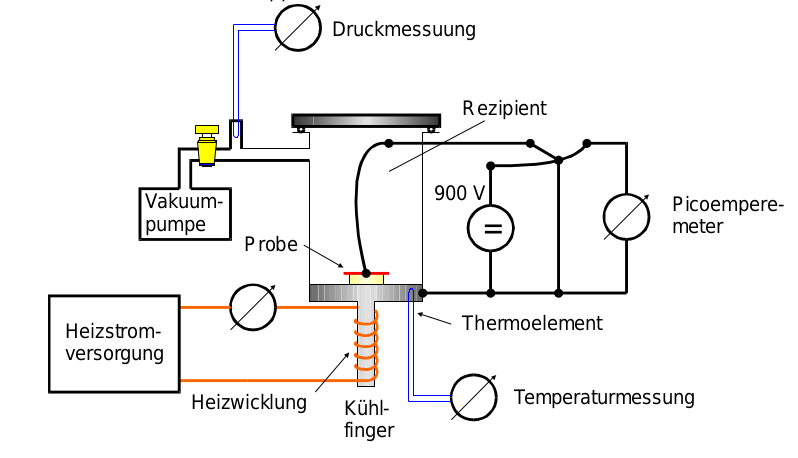
\includegraphics[scale=0.4]{bilder/aufbau.png}
	\caption{Schematischer Aufbau der Apparatur. \cite{AP}}
	\label{fig:aufbau}
\end{figure}
%
Die Probe befindet sich in einem Rezipienten auf dem Boden des Probenbehälters
mit Wärmeleitpaste verklebt. Die Messung wird im Vakuum
von ca. \SI{10^{-2}}{\milli\bar} durchgeführt, da
die Probe wasserempfindlich ist.
Die Durchführung kann nun wie folgt gegliedert werden.
%
\begin{enumerate}
	\item E-Feld ($U = \SI{600 - 900}{\volt}$) an die Probe bei
		einer Polarisationstemperatur von ca. $T_p = \SI{50}{\celsius}$ anschließen
		und ca. \SI{900}{\second} warten.
	\item Mit flüssigem Stickstoff auf ca. \SI{-40}{\celsius} bei eingeschaltetem
		E-Feld abkühlen.
	\item E-Feld abschalten und Kondensator ca. \SI{2}{min} kurzschließen.
	\item Picoamperemeter anschließen und den Strom beobachten bis er nahezu
		konstant ist
	\item Aufheizen mit konstanter Heizrate $b$ und entsprechende Ströme
		notieren.
\end{enumerate}
%
Dies wird für zwei Heizraten $b = \SI{1.5}{\K\per\second}$ und
$b = \SI{2}{\K\per\second}$ durchgeführt.
